\documentclass[a4paper,12pt]{article}
\usepackage[utf8x]{inputenc}
\usepackage{ucs}
\usepackage[T1]{fontenc}
\linespread{1.2}
\usepackage{amsmath,amssymb,amsthm,amsfonts,ulem}
\usepackage{courier, fourier}
\usepackage{clrscode3e}
\usepackage{mdwlist}
\setcounter{secnumdepth}{0}
\setcounter{tocdepth}{3}
\usepackage{todonotes}
\usepackage{hyperref}

\usepackage{subcaption}
\usepackage{float}
\usepackage{mdwlist}
\usepackage{wrapfig}
\usepackage{caption}
\newcommand{\graphicc}[4]{\begin{figure}[H] \centering
            \includegraphics[width={#1\textwidth}, keepaspectratio=true]{{#2}}
            \caption{{#3}} \label{#4} \end{figure}}

\title{Assignment 1 - Signal and Image Processing 2014}
\author{Martin Jørgensen}
\date{\today}

\begin{document}

\maketitle

\tableofcontents
\pagebreak

\section{Task 1.1}
\begin{figure}[h]
  \centering
  \begin{subfigure}[t]{0.3\textwidth}
    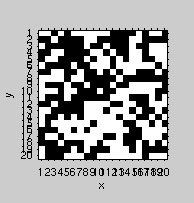
\includegraphics[width=\textwidth]{img/1_1_before.png}
    \caption{The randomly generated image.}
    \label{fig:1_1_before}
  \end{subfigure}%
  ~
  \begin{subfigure}[t]{0.3\textwidth}
    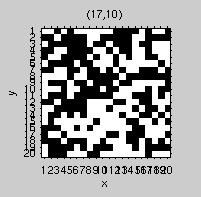
\includegraphics[width=\textwidth]{img/1_1_after.png}
    \caption{The randomly generated image with a blackened pixel as well as the
      coordinates.}
    \label{fig:1_1_after}
  \end{subfigure}
\end{figure}

This task was solved by generating a $20\times 20$ matrix of ones and
zeros. Then using ginput to retrieve the coordinates for a click and setting
that pixel to value $0$. Source code is in the appendix.

\section{Task 1.2}
To solve this I generated a $60\times 60$ image in the same way as Task 1.1, and
displayed it using the three different methods \texttt{imshow}, \texttt{image}
and \texttt{imagesc}. They are descriped in the list below.

\graphicc{0.95}{img/1_2.png}{The same image displayed using the different
  methods.}{fig:1_2}

\begin{description}
\item[\texttt{imshow}] Can take either a string with a filename/path, an image
  handle or a matrix as input and displays it as an image. It has a number of
  default attributes, such as disabling axis labels and ticks, and forcing
  square pixels by making the x and y axis have the same distance between ticks.
  It will also try to guess whether an image/matrix us in grayscale, RGB or
  binary.
\item[\texttt{image}] Takes a matrix as input which it will interpret as an
  image. The resulting image object will attempt to stretch to fill whatever
  window it is nested in, resulting in rectangular pixels. It will keep the tick
  marks along the images. Will use the active colormap instead of trying to
  guess what the data means.

\item[\texttt{imagesc}] Have the same behaviours as image, but will scale the
  image data to make use of the full colormap.
\end{description}

The source code is in the appendix.
\section{Task 1.3}

This task was solved by using a for loop and an array function to extract a
given bit for all pixels at once and order it into sub plots. See appendix for
source code.

\graphicc{0.95}{img/1_3.png}{The bit plances obtained from splicing
  \textit{cell.tif}}{fig:1_3}

Just like in the books Figure 1.3 on page 5, we see that the most significant
bits contain most of the coarse image information so the lower bits resembles
noise. Since this is a grayscale image where objects that er visible are whiter
(intensity close to 255) it makes sense that objects are visible in the higher
bit planes. Thw lower bit planes encompas only small variations in the visiblity
but a change in for isntance the 8'th bit will change the intensity with 128, or
half of the possible intensity.

\section{Task 1.4}
For this task I chose one of the sample pictures, the cookie monster
picture. (\textit{monster.jpg}). The code is very simple and can be found in the
appendix.

\graphicc{0.9}{img/1_4.png}{The HSV channels extracted from the original
  image.}{fig:1_4}

\section{Task 1.5}
The code used to generate the figures can be found in the appendix.
\graphicc{0.8}{img/1_5_downscale.png}{The Cookie monster image sized down using
  three different scales. The last one also ruins the aspect ratio of the
  image.}{fig:1_5_down}

In the upper right image, ther eis clear aliasing as the resolution falls and
``smooth'' edges can no longer be drawn. It is still possible to make out all
the details, evne though the curls in Cookie Monsters fur and the
ligh-reflections on the green lego brick is harder to make out.  In the lower
left image on Figure \ref{fig:1_5_down} several details are gone, the pupils in
Cookie Monsters eyes as well as the reflections on the lego block are almost
impossible to make out. The text on the jar is unreadable. The lower right image
in the same figure does not loose the details, but because the aspext-ratio is
skewed, some details like the text on the jar is a bit hard to make out.

\graphicc{0.8}{img/1_5_upscale.png}{Results when scaling up a low resolution
  image, in this case the original is the cookie monster picture scaled
  down.}{fig:1_5_up}

The upper right image in Figure \ref{fig:1_5_up} is created by giving all the
new pixels the same value as the pixel that is nearest their position in the
original image. This essentially ``stretches'' all the pixels and gives a very
jagged look. When comparing it to the original they're identical since they're
displayed in the same size. The two lower figures are taken by giving new pixels
a value based on the average value in their neighborhood in the original
image. ($2\times 2$ and $4\times 4$ neighborhoods respectively.) The edges gets
a lot softer and less jagged, but the image gets a very fussy quuality to it, as
if the camera was out of focus.

\section{Task 1.6}
The code for this task is shown in the appendix.

\graphicc{0.4}{img/1_6.png}{Measurements (in pixels) of the railway sleepers.}{fig:1_6}

Figure \ref{fig:1_6} shows the measurements of the sleepers on the railway. 2 parallel lines were
added at the end of the sleepers in order to facilitate easier measurements of the sleepers that are
further into the background, since these were blurry.

The first measures sleepers is $165,5$ pixels across. The second is $77.5$ px and the third is
$35.75$ px. It is impossible to recreate the $(X,Y,Z)$ positions of the sleepers without any more information.
We lack both focal length, and some information about positions in the scene. We can use the rate at
which the sleepers get shorter, i.e. how fast the lines that go to the vanishing point converges, to
make some assumptions about how ``wide'' things in the picture are along the $x$-axis, but apart from
that there is little we can do.

Example, I measured the distance between the two ``parallel'' lines to be $4.5$ px, at the same
distance as the first white house, the wall of the white house is roughly $4.5$ px tall and $25.38$ px wide.
Knowing that for every $4.5$ pixel we have roughly $2.5$ meters, the wall must be around $2.5$ meters
tall and $14.1$ meters long. ($\frac{25.38px}{4.5px}2.5m = 14.1m$). This assumes that the wall is
somewhat parallel to the camera.
\section{Task 1.7}
\graphicc{0.95}{img/1_7.png}{The results fo the different methods and
  operations.}{fig:1_7}

The two first pictures in Figure \ref{fig:1_7} is the result of two methods of
adding images. Since the image is bound by the 8bit intensity limit, they
produce the same result. The add the intensities of the images together, bound
it at 255 and displays it. When letting \texttt{imadd} (upper right image) give
16 bit output, the result is vastly different. The increased number of different
shades means that values that become higher than 255 does not jost go white. The
images are showed with \texttt{imagesc} in order to increase the visibility of
the number of intensities.

For the last two images, just like the first, there is no
difference. Intensities cannot go below 0, and as such they just go black. It is
not possible to specify 16bit output for \texttt{imsubtract}, but it would not
help, since we cannot display a negative intensity.

\section{Task 1.8}
The code for this task can be found in the appendix.

\graphicc{1.2}{img/1_8.png}{The differences between frames of the cell
  ``animation''.}{fig:1_8}

The difference is maxed by showing the images using \texttt{imagesc} which will
scale it to use the entire grayscale colormap. This allows us to see details
more clearly. The result from the operation is that pixels that change a lot,
gets a stronger (whiter) color, so areas with much change will ``light
up''. This can be usefull for motion tracking, if the background is largely
static, like in this image, it i easy to track objects moving over it, simply
follow the white areas around.

\section{Task 1.9}
The code for both the multiplication function and the experiment can be found in the appendix.

\graphicc{0.5}{img/1_9.png}{}{fig:1_9}



\appendix
\section{Appendix}
\subsection{Code for Task 1}
\codefig{p1}{../p1.m}{1}{39}{Code for producing the figure for the first task.}

\subsection{Code for Task 4}
\subsubsection{\texttt{LSI} function}
\codefig{p41}{../LSI.m}{1}{4}{LSI function.}
\subsubsection{Creating the figure}
\codefig{p42}{../p4.m}{1}{18}{Code for producing the figure for the fourth task.}

\subsection{Code for Task 5}
\subsubsection{\texttt{ILSI} function}
\codefig{p51}{../ILSI.m}{1}{10}{ILSI function.}
\subsubsection{Creating the figure}
\codefig{p52}{../p5.m}{1}{28}{Code for producing the figure for the fourth task.}



\end{document}
